% Header
\renewcommand\evenpagerightmark{{\scshape\small Chapter 3}}
\renewcommand\oddpageleftmark{{\scshape\small Muon Phase-II Upgrade}}

\renewcommand{\bibname}{References}

\hyphenation{}

\chapter[Muon Phase-II Upgrade]%
{Muon Phase-II Upgrade}
\label{chapt:3}
		
	The very first proton beam successfully circulated in the LHC in September 2008 directly followed by an incident leading to mechanical damage that would delay the LHC program for a year until November 2009, the very first collisions at a center-of-mass energy of \SI{7}{TeV} taking place in March 2010. The energy of the beam would be increased after a \acf{LS1} starting early 2013 after less than 3 years of data taking. Nevertheless, this first data taking period at only \SI{7}{TeV} was sufficient to claim the discovery of a new particle compatible with the Higgs boson in July 2012. During the 2 years of shutdown, the upgrade of the accelerator allowed for several maintainances along the beam pipes, repair and consolidation of magnet connection and high-current splices. But not only the LHC was upgraded. Indeed, the experiments at the 4 collision points also took the advantage of this time to upgrade their system in prevision of the next LHC run (Run-II) until 2018 and the \acf{LS2} as the luminosity and energy of the beam would be continuously increasing. By the end of Run-II, the luminosity will have reached twice its nominal value when the center-of-mass energy has already got close to its nominal value by reaching an historical \SI{13}{TeV} for the first time in 2017.
	
	The next long shutdown will occur at the end of this year and will again be the occasion for similar maintenance and consolidation in prevision of Run-III and the future upgrade of LS3. Still, the main occupation of LS2 on LHC side will be the upgrade of LHC injectors. On the experiments side, LHCb and ALICE will, in a very tight schedule, implement major upgrades while ATLAS and CMS will wait until LS3 to upgrade their detectors in prevision of high luminosity \textit{LHC-Phase-II}. ALICE main challenge is an upgrade of their apparatus to cope with the \SI{50}{kHz} $Pb-Pb$ collisions. Similarly, LHCb will upgrade their frontend readout electronics to cope with the full \SI{40}{MHz} collisions delivered by LHC. ATLAS will perform standard maintenance and CMS will focus on the urgent upgrade of the pixel detector and on the installation of new muon detectors in order to take profit of LS2 time to mitigate the upgrade of detectors forseen during LS3. Run-III will start in 2021 with the LHC at its nominal center-of-mass energy and will bring LHC-Phase-I to an end at the end of 2023. By then the luminosity will only increase to reach 2.5 times the nominal luminosity but during these 3 years of run, the LHC will deliver as much integrated luminosity as what what brought during the almost 7 years of both Run-I and II of data taking. Phase-I will end with an overall \SI{300}{fb^{-1}} delivered.\\

\section{\acl{HL-LHC}}
\label{chapt3:sec:HL-LHC}
	
	\begin{figure}[H]
		\begin{subfigure}{\linewidth}
			\centering
			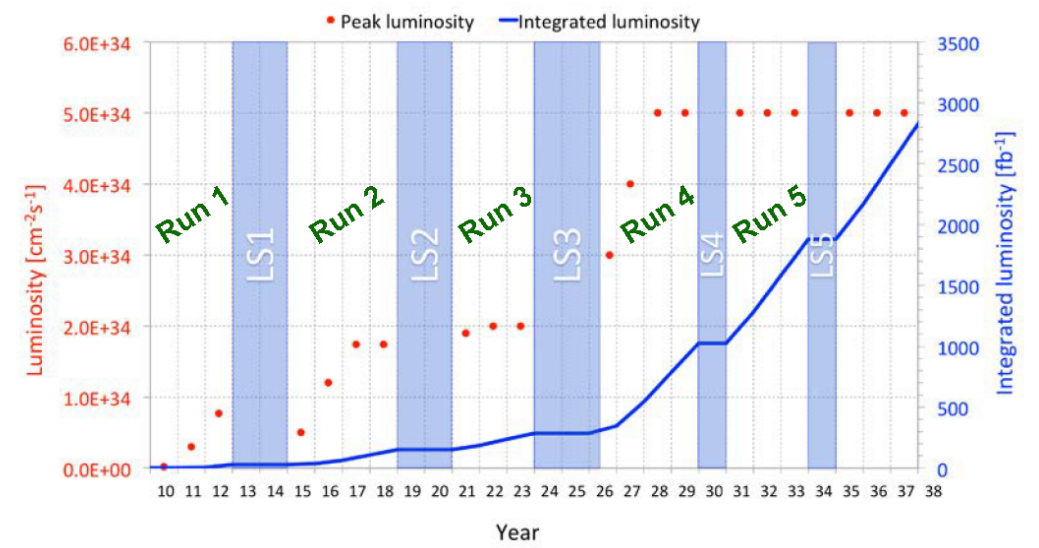
\includegraphics[width=\plotwidth]{fig/chapt3/HL-LHC-nominal.png}\\
			\caption{\label{fig:HL-LHC-Timeline:A}}
		\end{subfigure}
		\begin{subfigure}{\linewidth}
			\centering
			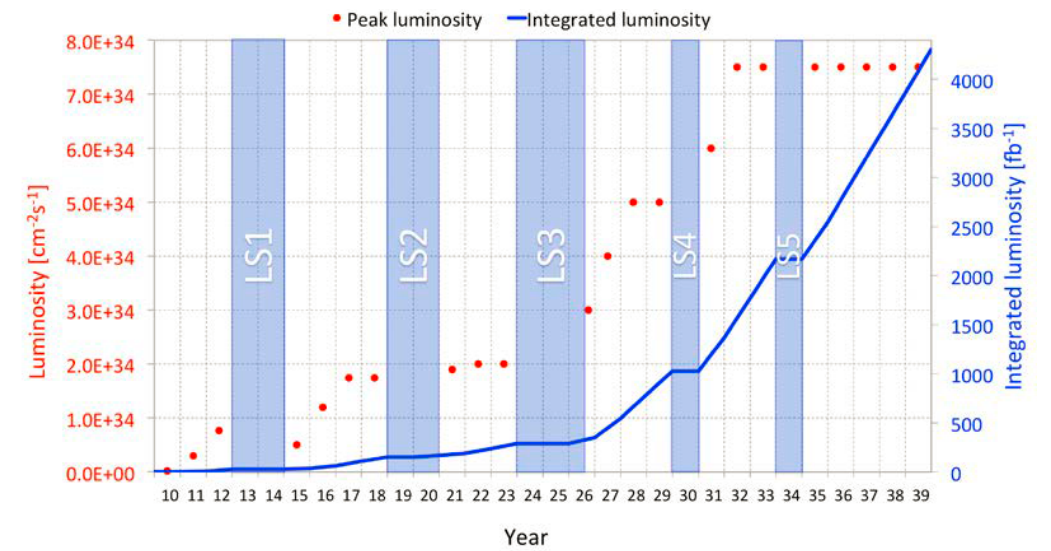
\includegraphics[width=\plotwidth]{fig/chapt3/HL-LHC-ultimate.png}
			\caption{\label{fig:HL-LHC-Timeline:B}}
		\end{subfigure}
		\caption{\label{fig:HL-LHC-Timeline} Detailed timeline projection of for LHC and HL-LHC operation until 2039 showing the evolution of the instanteneous and integrated luminosity as designed (Figure~\ref{fig:HL-LHC-Timeline:A}) and in the ultimate case where the instantaneous luminosity is increased to $7.5\times10^{34}$ \si{cm^{-2}s^{-1}} (Figure~\ref{fig:HL-LHC-Timeline:B})~\cite{HLLHC2017,HLLHCPDR}.}
	\end{figure}
		
	After approximately 15 years of operation, the LHC will undergo a new series of upgrade during the LS3 in order to boost its discovery potential as showed in Figure~\ref{fig:HL-LHC-Timeline}. This moment onward is what is referred to HL-LHC or Phase-II. The goal is to aim for a luminosity 5 to 7 times stronger than the nominal one trying to reach even 10 times this value if possible. Increasing the luminosity means that the beam size at the collision points needs to be reduced to boost the number of collisions per bunch crossing. For this purpose, new focusing and bending magnets, and collimators will be installed at the collision points as well as newly developed \textit{"crab cavities"} that will tilt the particle bunches just prior to the collisions by giving them transverse momentum and thus increasing their meeting area. In addition, the full proton injection line will be upgraded.
	
	Over its full lifetime, the HL-LHC is expected to deliver an outstanding integrated luminosity of \SI{3000}{fb^{-1}} leading, in the case of Higgs studies to measuring the couplings of the boson to a precision of 2 to 5\% thanks to the estimated 15 millions of Higgs created every year providing a more precise measurement of potential deviations from the theoretical predictions. SUSY and heavy gauge boson studies would also see their mass range limits pushed away by at least \SI{1}{TeV} and could lead to a new breakthrough. SUSY is a particularly important topic as it could give an answer to why the Higgs boson can stay so light while coupled to heavy particles by introducing the contributions of the super partners on top of providing dark matter candidates. Finally, the increase of luminosity will give the possibility to investigate "exotic" mode like for example the models introducing extra dimensions to explain the hierarchy problem.
	
	On the experiments side, the \acf{PU} will be increased up to 150 to 200 interactions per bunch crossing in ATLAS and CMS, making necessary an strong upgrade of the trigger system and of the inner trackers and of the calorimeters. Both ATLAS and CMS will also need to upgrade the muon trigger at the level of the endcaps mainly focusing on the coverage near the beam line in order to increase the detection acceptance and event selection. Moreover, the increased luminosity will also lead to an increased background rate and a faster ageing of the detectors. This PhD work takes place into this very specific context of muon detector consolidation and certification for the HL-LHC period in order to provide the CMS experiment with robust new detectors and confirm that the present system will survive through the next 20 years of HL-LHC.
	
\section{Muon system requirements through HL-LHC}
\label{chapt3:sec:requirements}

	\begin{figure}[H]
		\centering
		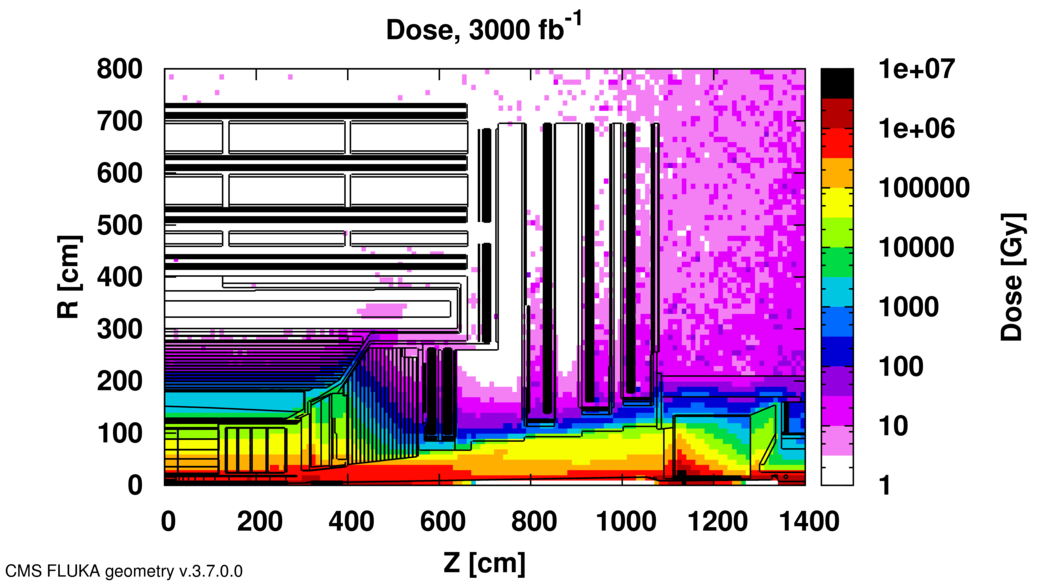
\includegraphics[width=0.7\textwidth]{fig/chapt3/HL-LHC-Dose.png}
		\caption{\label{fig:Dose} Absorbed dose in the CMS cavern after an integrated luminosity of \SI{3000}{\femto\per\barn}. Using the interaction point as reference, R is the transverse distance from the beamline and Z is the distance along the beamline.}
	\end{figure}

	The end of 2018 will mark the beginning of LS2 and the start of Phase-II upgrade activities. From the HL-LHC period onwards, i.e. past LS3, the performance degradation due to integrated radiation as well as the average number of inelastic collisions per bunch crossing, seen as pile-up into the detectors' readout that far exceeds this of the original LHC plans, will rise substantially and become a major challenge for all of the LHC experiments, like CMS, that were forced to address an upgrade program for Phase-II~\cite{PHASEIITP}. Dealing with the data from the muon detectors will force to upgrade the detectors and electronics towards the most recent technologies. Simultaneously, this will push new latency requirements onto the Level-1 trigger and the \acf{DAQ} that will only be fulfilled by upgrading the system with electronics having deeper buffering and faster processing. Simulations of the expected distribution of absorbed dose in the CMS detector under HL-LHC conditions show, in Figure~\ref{fig:Dose}, that detectors placed close to the beam line will have to withstand high irradiation, the radiation dose being of the order of a few tens of \si{Gy}.
	
	\begin{figure}[H]
		\centering
		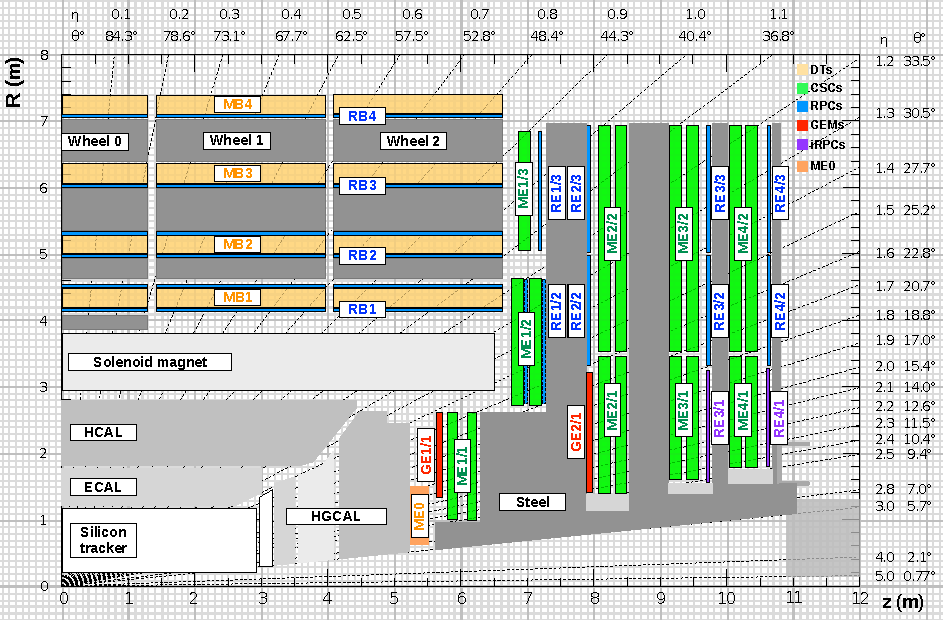
\includegraphics[width=0.7\textwidth]{fig/chapt3/Phase2_Muon_quadrant.pdf}
		\caption{\label{fig:P2Quadrant} A quadrant of the muon system, showing DTs (yellow), RPCs (blue), and CSCs (green). The locations of new forward muon detectors for Phase-II are contained within the dashed box and indicated in red for GEM stations (ME0, GE1/1, and GE2/1) and dark blue for improved RPC (iRPC) stations (RE3/1 and RE4/1).}
	\end{figure}
	
	While only the RPCs' electronic system is able to operate under Phase-II requirements, DTs and CSCs will need to improve their trigger accept rate and latency to ensure that Level-1 trigger threshold stays at the same level~\cite{LEVEL1IR}, and DAQ data transfer rate, that respectively need to achieve a minimum of \SI{500}{kHz}, get down to \SI{12.5}{\micro s}~\cite{CMSIITP}, and increase to \SI{1082}{Gbit/s} DTs and to \SI{1026}{Gbit/s} for CSCs. As of today, the Level-1 trigger accept rate of DTs doesn't reach \SI{300}{kHz} while this of CSCs is bellow \SI{250}{kHz} but the foreseen upgrades are expected to increase the rate way beyond the requirement in the of DTs and up to \SI{4}{MHz} for CSCs~\cite{PHASEIITP}.
	
	The \acf{MiC1} used by DTs don't allow for high enough trigger rate. In addition to this problem, it was showed that these electronics contain components that are not radiation hard enough to sustain HL-LHC conditions and thus, a too large number of channels may fail due to radiations. On the other hand, CSCs showed that there electronics would be able to live through the 10 years of Phase-II but the limited buffer depth might cause memory overflows and readout inefficiencies with a fraction of event loss ranging from 5 to 10\% depending on the expected background. Thus the replacement of CSCs' \acf{CFEBs} by digital ones, DCFEBs, with deeper buffer would solve the problem and satisfy HL-LHC requirements. Moreover, a lack of FPGA memory ressources is feared for CSCs' \acf{ALCTs} and the boards that were not already upgraded during LS1 will need to be replaced, also ensuring that the out bandwidth will be sufficient for the expected high data rate. Finally, all these new DT and CSC electronics will be connected to the trigger electronics via optical links to ensure a faster communication~\cite{PHASEIITP}.\\

	The increase of irradiation close to the beam line will affect the background rate seen by the muon detectors in this area and tracking muons will prove to be difficult as this region is not yet equipped with all the detectors that were already foreseen for Phase-I. Improving this situation will come with the increase of hit numbers recorded along the particle track to reduce the ambiguity on muon versus background detection. Moreover, the measurement of small production cross-section and/or decay branching ratio processes, such as the Higgs boson coupling to charge leptons, and in particular to muons, or the $B_s \longrightarrow \mu^+\mu^-$ decay, is of major interest and specific upgrades in the forward regions of the detector will be required to maximize the physics acceptance to the largest possible solid angle.
	
	To ensure proper trigger performance within the present coverage, the muon system will be completed with new chambers. Figure~\ref{fig:P2Quadrant} shows the addition of \acf{GEM} and \acf{iRPC} in the pseudo-rapidity region $1.6<\vert\eta\vert<2.4$ to complete the redundancy of the already existing CSCs as originally scheduled in the CMS Technical Proposal~\cite{CMSTP}. A first step into this direction will be taken by installing GEMs on the first endcap disk in position GE1/1 during LS2, during which preparations for the future installation of more GEMs and RPCs will take place by installing the needed services. During the YETS following LS2, iRPCs will be installed on the third and fourth endcap disks in position RE3/1 and RE4/1, and more GEMs will equip the second endcap in position GE2/1 and the inner layer, closest to the HCAL endcap called ME0 during LS3, finally completing the redundant coverage of the muon system and extending it a little by extending the reach to \psrape{2.8}, the redundancy in the region \psrapr{2.4}{2.8} being maintained by the 6 GEM layers contained in each ME0 detector that provide enough tracking points to efficiently reject neutron-induced background.
	
	Nevertheless, the region beyond \psrapg{2.8} and extending to \psrape{5.0} only is covered by the forward HCAL detectors and lack redundant muon detector coverage. Extensions of the tracker in the context of HL-LHC will increase its coverage up to \psrape{4.0} but the identification of muons and measurement of their energy with reasonable precision only using the tracker is nearly impossible. Thus, this increased tracker coverage range needs to be put in parallel with a matching muon detector and will open doors to multi-lepton final states in which leptons are likely to have a a low transverse momentum and to be found near the beam line.\\
	
	Finally, as the muon system is composed only of gaseous detectors, strong environmental concerns have risen over the last years as the European directives will restrict the use of fluorine based gas mixtures. Both the CSC and RPC subsystems, using $CF_4$, $C_2H_2F_4$, or $SF_6$, will need to adapt their working gas in order to strongly reduce the greenhouse potential of the mixtures released into the atmosphere due to gas leaks.
	
\section{Forseen upgrades of DTs and CSCs}
\label{chapt3:sec:DTCSCP2}

\section{New detectors and increased acceptance}
\label{chapt3:sec:GEMRPC}

	RPCs are used by the CMS first level trigger for their good timing performances. Indeed, a very good bunch crossing identification can be obtained with the present CMS RPC system, given their fast response of the order of \SI{1}{ns}. In order to contribute to the precision of muon momentum measurements, muon chambers should have a spatial resolution less or comparable to the contribution of multiple scattering~\cite{MUONTDR}. Most of the plausible physics is covered only considering muons with $p_T<$\SI{100}{GeV} thus, in order to match CMS requirements, a spatial resolution of $\mathcal{O}$(few $\mathrm{mm}$) the proposed new RPC stations, as shown by the simulation in figure~\ref{fig:MultiScat}. According to preliminary designs, RE3/1 and RE4/1 readout pitch will be comprised between 3 and \SI{6}{mm} and 5 $\eta$-partitions could be considered.

\begin{figure}[H]
	\centering
	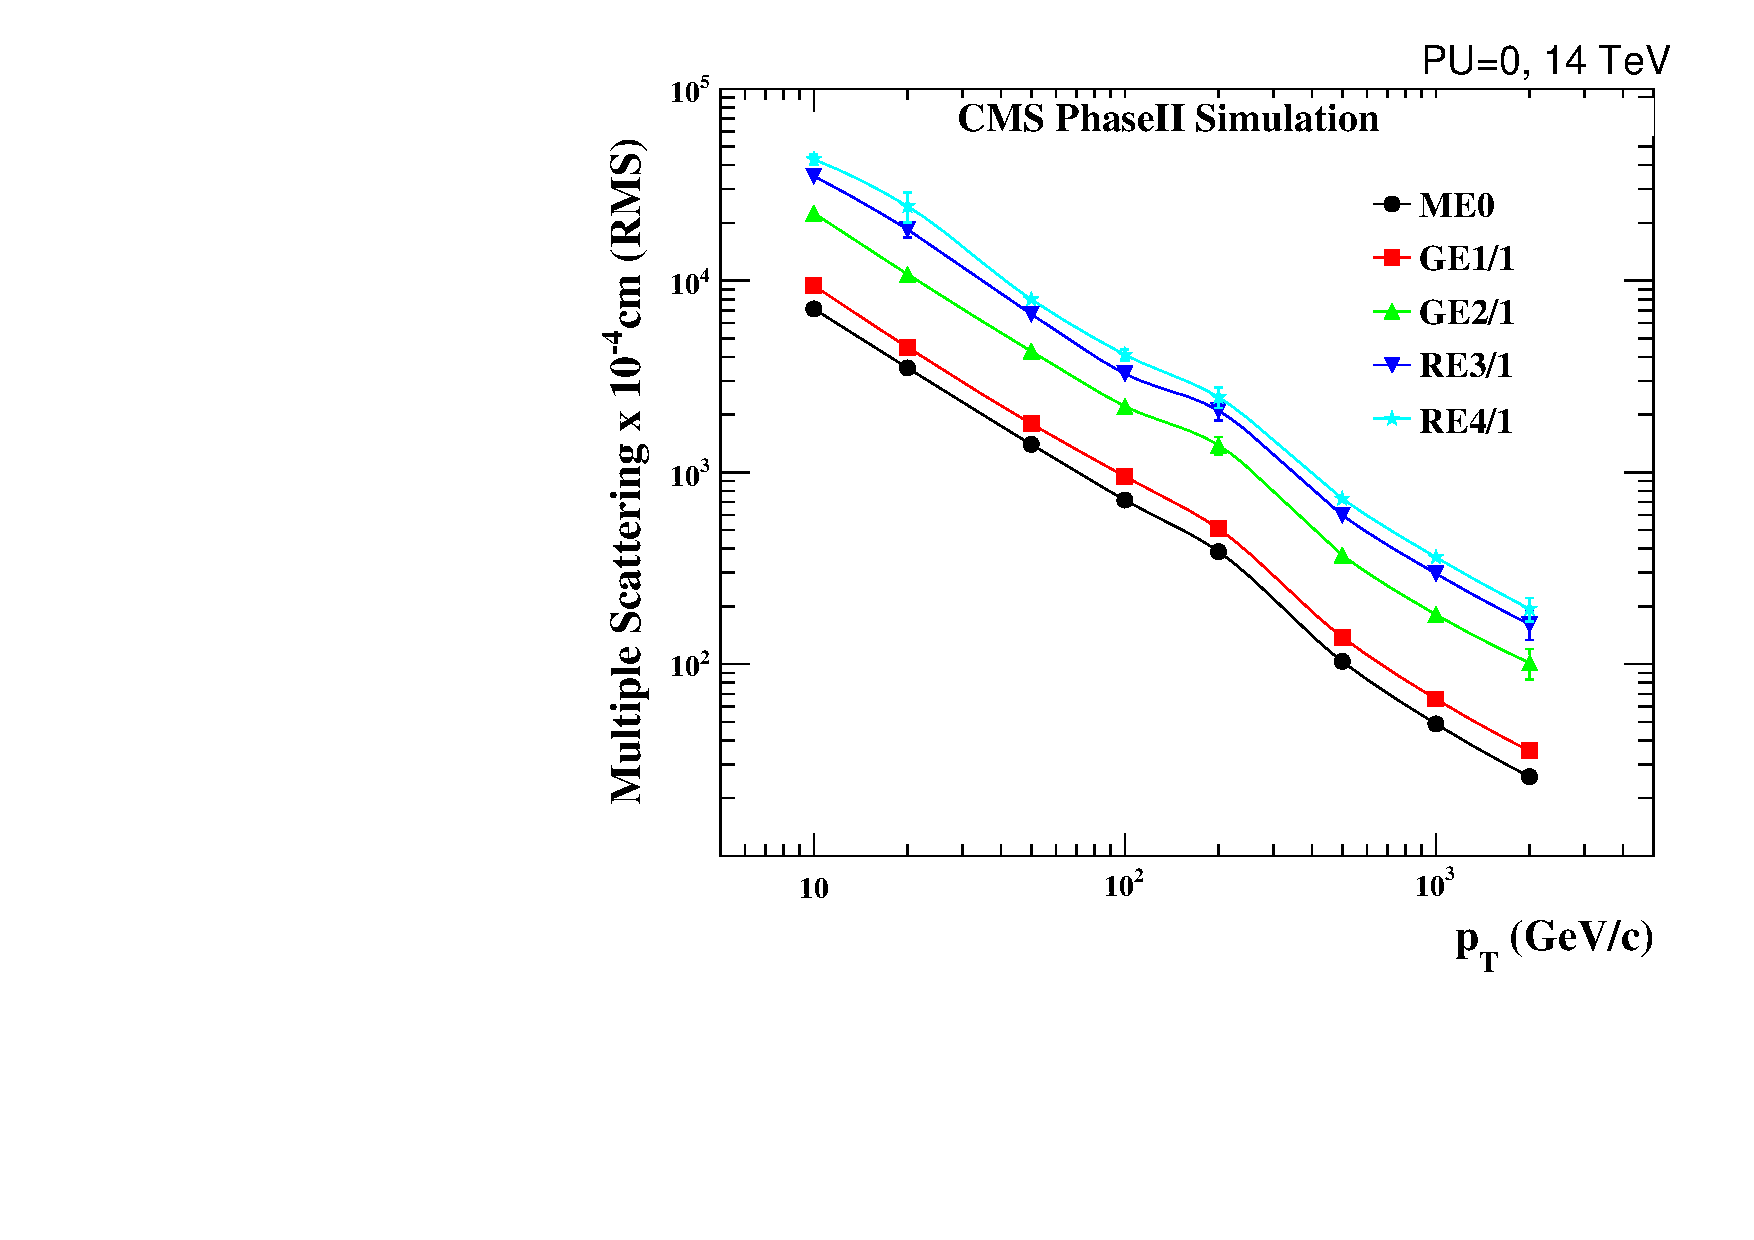
\includegraphics[width=0.6\textwidth]{fig/chapt3/MS_allstations.pdf}
	\caption{\label{fig:MultiScat}  RMS of the multiple scattering displacement as a function of muon $p_T$ for the  proposed forward muon stations. All of the electromagnetic processes such as bremsstrahlung and magnetic field effect are included in the simulation.}
\end{figure}

\section{Implications of the different upgrades on the Level-1 Trigger}
\label{chapt3:sec:L1tP2}

\section{Improvement of physics performance}
\label{chapt3:sec:Physics}

\clearpage{\pagestyle{empty}\cleardoublepage}